% !TEX root = ../main.tex
% SECTION 6: LAGER, LAGERUNGEN UND SCHMIERUNG
% Inhalt: Liv Erne, Silvio Seiz — Form: ZSF-Template-Rework
% ============================================================

\StartChapter[ch:lager]{Lager, Lagerungen und Schmierung}

\SubsectionBar[sec:wälzlager]{Wälzlager}
\ZSFindex[walzlager]{Wälzlager}

\begin{defbox}[Wälzlager]
Bezeichnet das eigentliche mechanische Bauteil mit \ZSFkeyword{Innenring}, Käfig, Dichtung, \ZSFkeyword{Aussenring} und \ZSFkeyword[Walzkorper@Wälzkörper]{Wälzkörper}.
Verschiedene Formen mit unterschiedlichen Kontaktgeometrien, je nach Lastfall.
\end{defbox}

%\ZSFfig{graphics/rolling_bearing_deep_groove_radial_axial_load.png}{Wälzlager}{}
\begin{splitbox}[0.44]
  \begin{figbox}[Wälzlager-Bauformen]
    \centering
    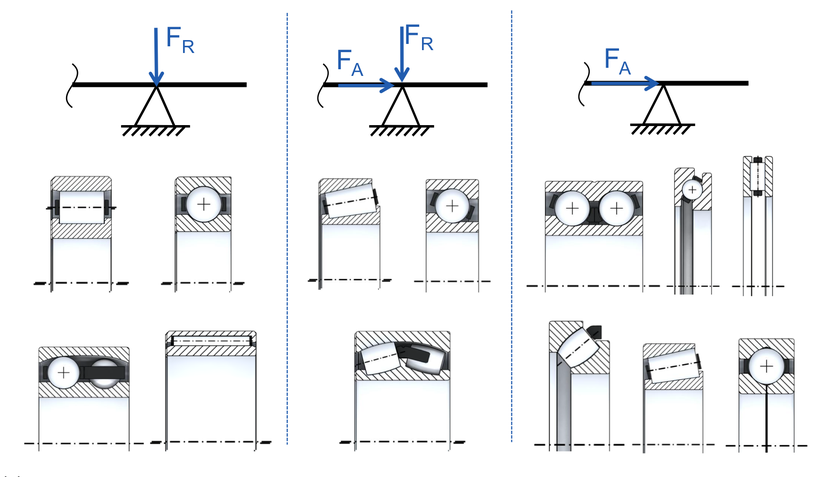
\includegraphics[width=\linewidth,keepaspectratio]{graphics/rolling_bearing_types_load_cases.png}% chktex 25
  \end{figbox}
\tcblower
  \begin{warnbox}[Lagerschäden]
    \begin{factlist}
    \item Wälzkörpereindrücke und Schlupfspuren bei falscher statischer Belastung.
    \item \ZSFkeyword{Pitting} und Fremdkörperüberrollung wenn Fremdstoffe in den Reibkontakt gelangen.
    \end{factlist}
  \end{warnbox}
\end{splitbox}
\ZSFindex[lagerschaden]{Lagerschäden}

\SubsectionBar[sec:lagerungen]{Lagerungen}
\ZSFindex{Lagerung}

\begin{tablebox}[Lagerungen: Definition, Funktion \& Bauarten]
  \ZSFReadableOn
  \setlength{\leftskip}{\ZSFspaceS}%
  \setlength{\rightskip}{\ZSFspaceS}%
  \vskip\ZSFspaceXS
  \textbf{Def:} Baugruppe, die ein Bauteil mit $\ge 2$ Lagern stützt/führt. \\
  \textbf{F1:} Rotation zulassen, Reibungsverluste reduzieren. \hfill
  \textbf{F2:} Freiheitsgrade begrenzen, Kräfte ableiten.
  \par
  \vskip\ZSFspaceXS
  \setlength{\leftskip}{0pt}%
  \setlength{\rightskip}{0pt}%
  \renewcommand{\arraystretch}{1.1}%
  \setlength{\tabcolsep}{2.0pt}%
  \begin{ZSFtable}[\ZSFfontTableDense]{Y{0.50} Y{1.30} Y{1.20}}
    \ZSFheaderRow 
    \ZSFhead{Lagerungen} & \ZSFhead{+} & \ZSFhead{--} \\
    \textbf{Fest-Los} & 
    $\cdot$ Wechselnde Axiallast \newline 
    $\cdot$ Eindeutige Position durch Festlager \newline 
    $\cdot$ Längenausgleich durch Loslager \newline 
    $\cdot$ Statisch bestimmt & 
    $\cdot$ Zusätzl. Bauteile \& Fertigungsschritte \\
    
    \textbf{Schwimmend} & 
    $\cdot$ Keine zusätzl. Bauteile oder Fertigungsschritte \newline 
    $\cdot$ Längenausgleich möglich & 
    $\cdot$ Axiales Spiel $\Rightarrow$ keine wechselnde Axiallast \newline 
    $\cdot$ Axiallast $\Rightarrow$ keine hohe Genauigkeit \\
    
    \textbf{Angestellt (X/O)} & 
    $\cdot$ Aufnahme hoher Axialkräfte \newline 
    $\cdot$ Hohe Positionsgenauigkeit \newline 
    $\cdot$ Gute Aufnahme von Kräften zw. Lagern & 
    $\cdot$ Sicherstellen der def. Vorspannung $\rightarrow$ hohe Kosten \newline 
    $\cdot$ Kein Längenausgleich $\rightarrow$ Schäden
  \end{ZSFtable}%
  
  \ZSFgapXS
  \setlength{\tabcolsep}{2.0pt}%
  \begin{ZSFtablePlain}[\ZSFfontTableDense]{Z{1.0} Z{1.0} Z{1.0} Z{1.0}}
    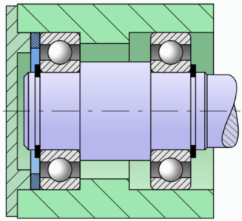
\includegraphics[width=0.95\hsize,height=1.45cm,keepaspectratio]{graphics/lagerung_fest_los.png} &
    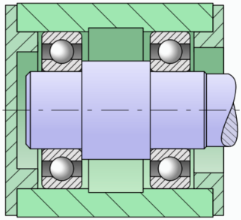
\includegraphics[width=0.95\hsize,height=1.45cm,keepaspectratio]{graphics/lagerung_schwimmend.png} &
    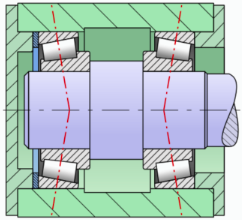
\includegraphics[width=0.95\hsize,height=1.45cm,keepaspectratio]{graphics/lagerung_angestellt_x.png} &
    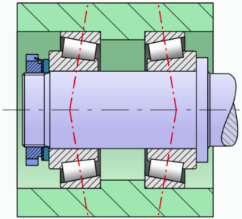
\includegraphics[width=0.95\hsize,height=1.45cm,keepaspectratio]{graphics/lagerung_angestellt_o.png} \\
    \TableTitle{Fest-Los} &
    \TableTitle{Schwimmend} &
    \TableTitle{Angestellt (X)} &
    \TableTitle{Angestellt (O)}
  \end{ZSFtablePlain}%
\end{tablebox}
\ZSFindex{Fest-Los-Lagerung}



\SubsubsectionBarOnNewColumn{Passungen / Punkt- und Umfangslast}
\ZSFindex{Punktlast}
\ZSFindex{Umfangslast}
\ZSFindex{Lebensdauer}

\begin{runintext}
Spiel-, Übergangs- und Presspassungen \ZSFref{sec:toleranzfeldbilder} beim Konstruieren von Wälzlagern zwischen Innenring und Welle, sowie Aussenring und Gehäude.
\end{runintext}

\ZSFfig[1.0]{graphics/rolling_bearing_point_circumferential_load_fit.png}{Punkt- und Umfangslast}{} % chktex 25

\begin{formulabox}[Lebensdauer und Tragfähigkeit]
\formulasources{$\ZSFbearP$:~\ZSFsource{bestimmen mit}{proc:lager-p}}
\[ \ZSFbearS = \dfrac{\ZSFbearR}{\ZSFbearB} \qquad \ZSFbearSZero = \dfrac{\ZSFbearCZero}{\ZSFbearPZero} \]
\[ \ZSFbearLTen = (\dfrac{\ZSFbearC}{\ZSFbearP})^\ZSFbearExp \qquad \ZSFbearLTenH = (\dfrac{\ZSFbearC}{\ZSFbearP})^\ZSFbearExp \cdot \dfrac{10^6}{60\cdot \ZSFbearN} \]
\[ \ZSFbearCerf = \ZSFbearP\cdot \sqrt[\ZSFbearExp]{\dfrac{60\cdot \ZSFbearN\cdot \ZSFbearLTenH}{10^6}} \]
\formulanote{$\ZSFbearLTen$:~nom. Lebensdauer \ $\cdot$ \ $\ZSFbearSZero$:~stat. Tragfähigkeit \ $\cdot$ \ $\ZSFbearCZero$:~stat. Tragzahl \\
$\ZSFbearPZero$:~stat. äquiv. Belastung \ $\cdot$ \ $\ZSFbearC$:~dyn. Tragzahl \ $\cdot$ \ $\ZSFbearP$:~dyn. äquiv. Tragzahl \\
$\ZSFbearExp$:~Lebensdauerexponent (Kugellager $\ZSFbearExp=3$, Rollenlager $\ZSFbearExp=10/3$)}
\end{formulabox}

\phantomsection\label{proc:lager-p}
\begin{procedure}[Dynamisch äquivalente Belastung $\ZSFbearP$ bestimmen]
\ProcStep{$\ZSFbearX$, $\ZSFbearY$, $\ZSFbearE$ bestimmen}{$\dfrac{\ZSFbearFZero\cdot \ZSFbearFa}{\ZSFbearCZero}\rightarrow Tabelle$ \ \ZSFmuted{$\dots\ZSFbearX, \ZSFbearY$ abhängig vom Lager}}
\ProcStep{Fallunterscheidung}{$\dfrac{\ZSFbearFa}{\ZSFbearFr} > \ZSFbearE \rightarrow \ZSFbearP = \ZSFbearX\cdot \ZSFbearFr + \ZSFbearY\cdot \ZSFbearFa$ \quad $\dfrac{\ZSFbearFa}{\ZSFbearFr} \leq \ZSFbearE \rightarrow \ZSFbearP = \ZSFbearFr$}
\end{procedure}

\SubsectionBar[sec:schmierung]{Schmierung}
\ZSFindex{Schmierung}

\begin{runintext}
\ZSFkeyword{Schmiermittel} wie Öle und Fette bilden auf den Oberflächen einen Film, der den direkten Kontakt von Stahl auf Stahl verhindert, um Reibung zu minimieren.
\end{runintext}

\begin{splitbox}[0.54]
  \begin{warnbox}[Beanspruchung \& Schädigung]
    \ZSFReadableOn
    \begin{factlist}
      \item \ZSFkeyword{Hertzsche Pressung}:~Höchste Beanspruchung knapp \ZSFhl{unter der Oberfläche} $\rightarrow$ Risskeime, \ZSFkeyword{Pitting} (Grübchen).
      \item \textbf{Verschleiss}:~Abrieb durch Schmutz/Mangelschmierung.
      \item \textbf{Korrosion}:~Rost/Stromdurchgang schädigt Laufbahnen.
    \end{factlist}
  \end{warnbox}
\tcblower
  \begin{figbox}[Stribeck-Kurve]
    \centering
    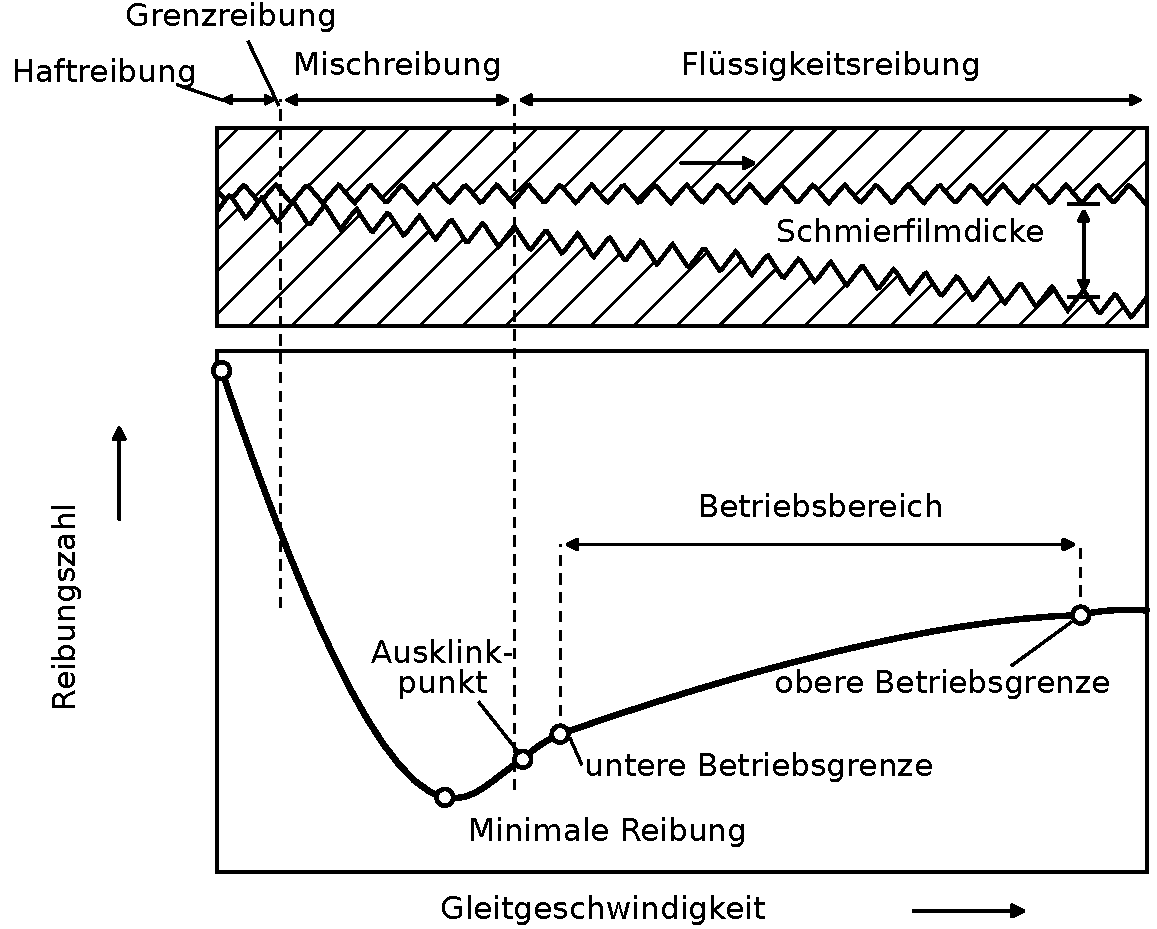
\includegraphics[width=0.98\linewidth,keepaspectratio]{graphics/stribeck.pdf}
  \end{figbox}
\end{splitbox}
\ZSFindex{Stribeck-Kurve}
